\section{Hashed Shading Algorithm}
%\subsection{Overview}

\begin{figure}[t]
  \usetikzlibrary{shapes.arrows, fadings}
  \definecolor{LightColor}{rgb}{1.0,0.901,0.805}

  \definecolor{tile0}{HTML}{DABDE4}
  \definecolor{tile1}{HTML}{B8DBF4}
  \definecolor{tile2}{HTML}{B5EDCD}
  \definecolor{tile3}{HTML}{FBEBA7}
  \definecolor{tile4}{HTML}{F9C1BB}
  \definecolor{tile5}{rgb}{1, 1, 1}

  \tikzstyle{array_element}=[rectangle,
                             minimum height=1cm, 
                             minimum width=1cm, 
                             minimum size=1cm,
                             draw=black,
                             rounded corners=2.5 ]
  \tikzstyle{grid_element}=[rectangle,
                            minimum height=1.5cm, 
                            minimum width=1.5cm, 
                            draw=black,
                            rounded corners=2.5 ]
  \tikzstyle{grid_element_big}=[rectangle, 
                               minimum height=2cm, 
                               minimum width=2cm, 
                               draw=black,
                               rounded corners=2.5 ]
 \tikzstyle{grid_element_bigly}=[rectangle, 
                               minimum height=3cm, 
                               minimum width=3cm, 
                               draw=black,
                               rounded corners=2.5 ]


\begin{adjustbox}{minipage=\textwidth, scale=0.5}
  \centering
  \begin{tikzpicture}
    \node at (-4.cm, 4cm) (light_list_name) [anchor=west] {\LARGE Global Light List:};
    \node at (-4.cm, 2cm) (light_list_name) [anchor=west] {\LARGE Light Index List:};
    \node at (-4.cm, -1.5cm) (light_list_name) [anchor=west] {\LARGE Octree:};
    \node at (2.75cm, -1.5cm) (light_list_name) [anchor=west] {\LARGE Spatial Hash Functions:};
    

    \foreach \l in {0,...,6} {
      \node at (1cm * \l + 1cm, 4cm) (light_\l) [array_element,fill={LightColor}] {$\mathbf{l}_\l$};
    }
    \node at (1cm * 7, 4cm) [array_element, fill={LightColor}, ] {};
    \node at (1cm * 7.325, 4cm) [rectangle,
                                 minimum height=1.2cm,
                                 minimum width=0.6cm,
                                 fill={white},
                                 draw=white] {};
    \node at (1cm * 7, 4cm) [rectangle,                    
                             minimum height=0.98cm, 
                             minimum width=0.2cm, 
                             shading = axis,
                             shading angle=90,
                             left color=LightColor ] {};
                             
    \node at (1cm * 7, 4cm) [rectangle, minimum height=1cm, minimum width=1cm] {$\dots$};

    \node at (1cm * 0, 2cm) [array_element,
                              fill={white}, ] {};
    \node at (1cm * -0.325, 2cm) [rectangle,
                                  minimum height=1.2cm,
                                  minimum width=0.6cm,
                                  fill={white},
                                  draw=white] {};
    \node at (1cm * 0, 2cm) [rectangle,
                              minimum height=1cm,
                              minimum width=1cm] {$\dots$};


    \foreach \i/\l in {0/0} {
      \node at (1cm * \i +1cm, 2cm) (light_index_\i) [array_element, fill={tile0}] {\l};
      \draw[-latex] (light_index_\i.north) -- (light_\l.south);
    }
    \foreach \i/\l in {1/0, 2/1, 3/4} {
      \node at (1cm * \i  +1cm, 2cm) (light_index_\i) [array_element, fill={tile1}] {\l};
      \draw[-latex] (light_index_\i.north) -- (light_\l.south);
    }
    \foreach \i/\l in {4/2, 5/4} {
      \node at (1cm * \i  +1cm, 2cm) (light_index_\i) [array_element, fill={tile2}] {\l};
      \draw[-latex] (light_index_\i.north) -- (light_\l.south);
    }
    \foreach \i/\l in {6/5} {
      \node at (1cm * \i  +1cm, 2cm) (light_index_\i) [array_element, fill={tile3}] {\l};
      \draw[-latex] (light_index_\i.north) -- (light_\l.south);
    }
    \foreach \i/\l in {7/3, 8/5, 9/6} {
      \node at (1cm * \i  +1cm, 2cm) (light_index_\i) [array_element, fill={tile4}] {\l};
      \draw[-latex] (light_index_\i.north) -- (light_\l.south);
    }
    \node at (1cm * 10  +1cm, 2cm) [array_element,
                              fill={white}, ] {};
    \node at (1cm * 10.325  +1cm, 2cm) [rectangle,
                                  minimum height=1.2cm,
                                  minimum width=0.6cm,
                                  fill={white},
                                  draw=white] {};
    \node at (1cm * 10  +1cm, 2cm) [rectangle,
                              minimum height=1cm,
                              minimum width=1cm] {$\dots$};

\node[inner sep=0pt] (level_0) at (-1.25cm,-5.5cm - 1cm)
    {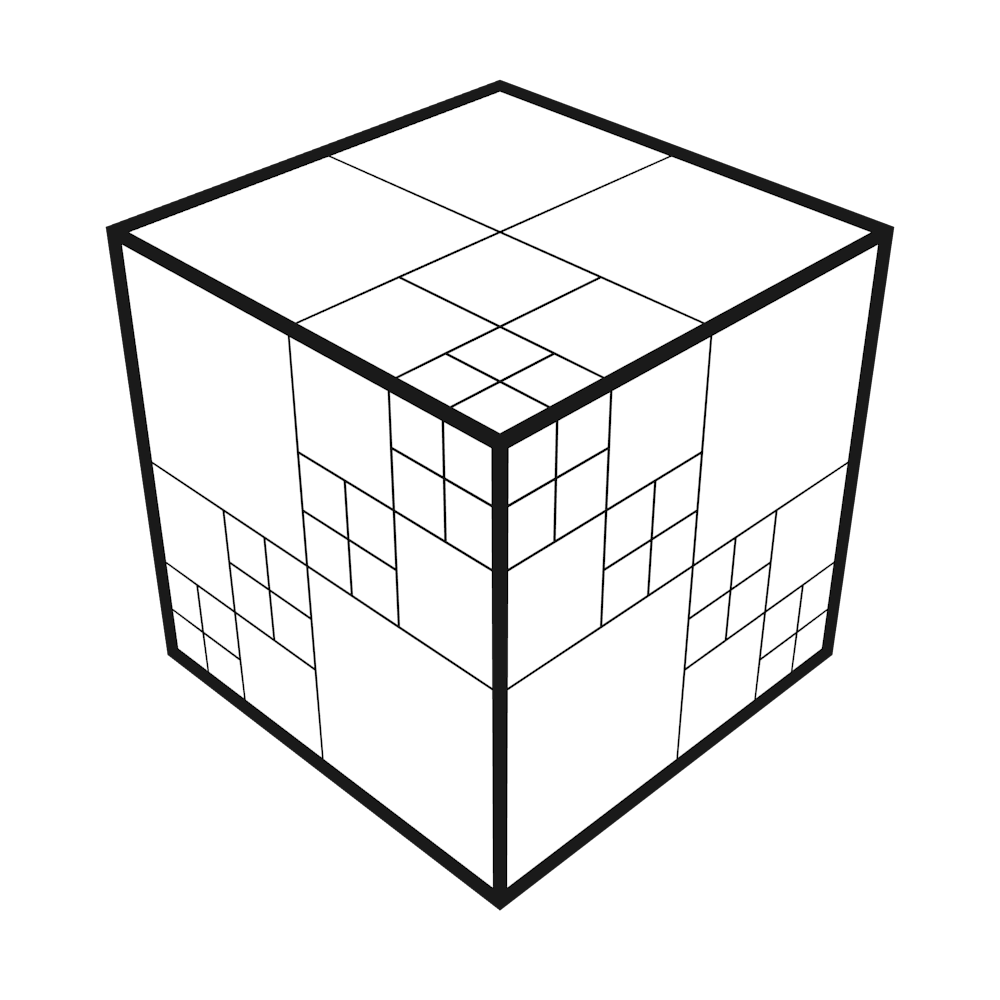
\includegraphics[width=6.5cm]{./img/raw/hs-datastructuren-overzicht/octree.png}};
    
\node at (4cm, -2.cm) {$\vdots$};
\node at (4cm, -10.5cm) {$\vdots$};




\node[inner sep=0pt] (level_0) at (4.0cm,-3cm  - 1.5cm)
    {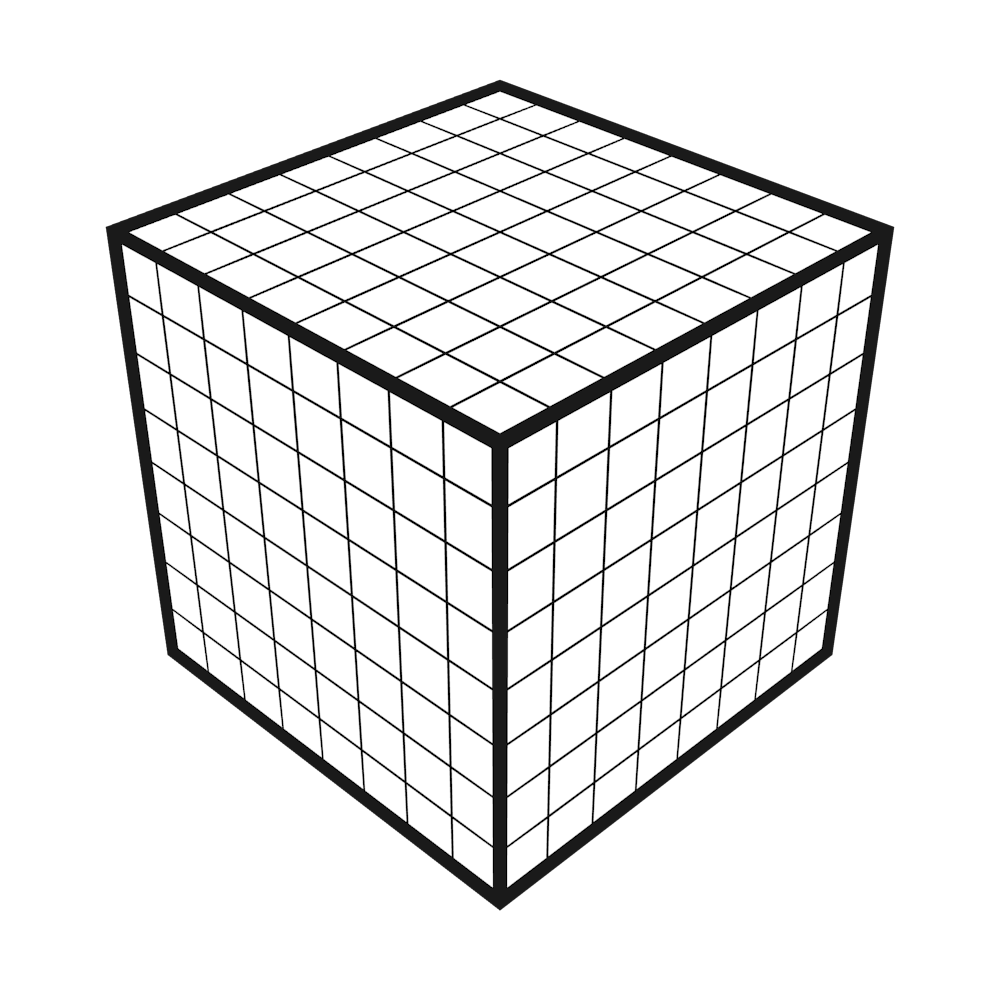
\includegraphics[width=3cm]{./img/raw/hs-datastructuren-overzicht/img1.png}};
\node[inner sep=0pt] (level_0) at (6.25cm,-2.75cm  - 1.5cm)
    {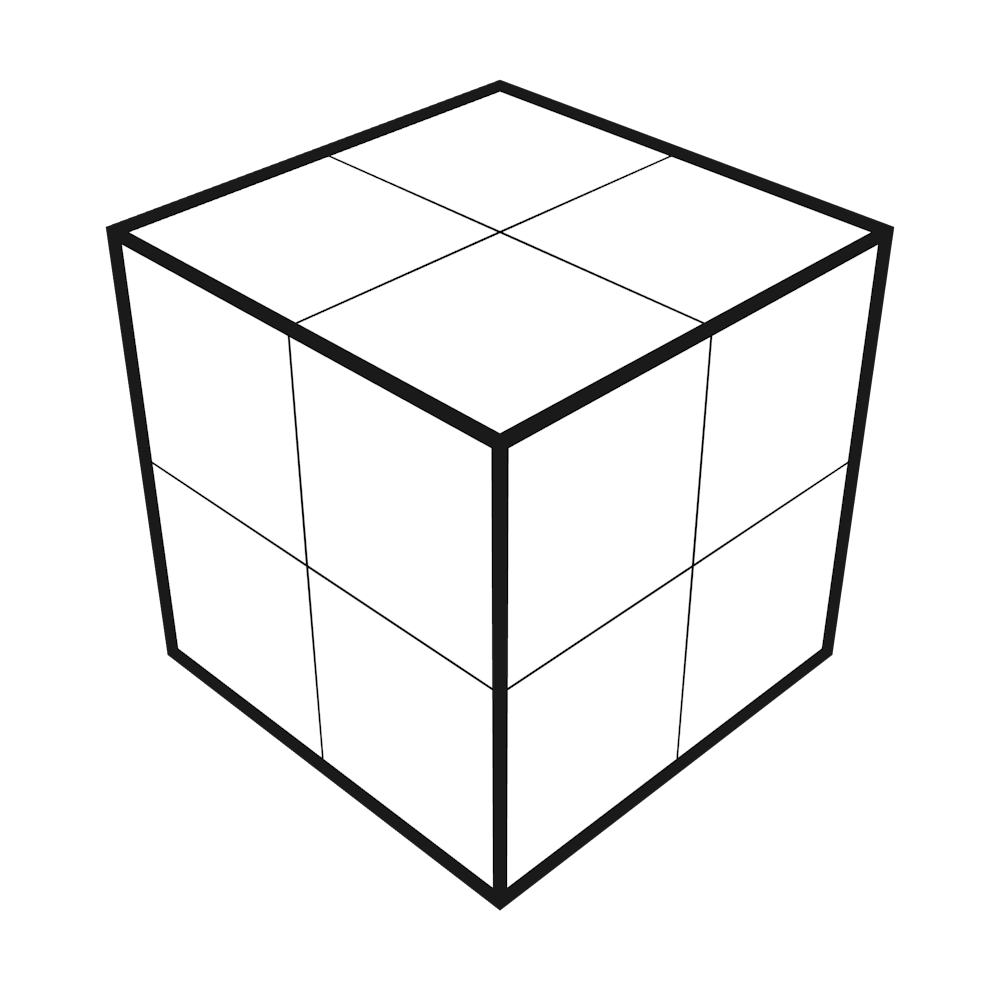
\includegraphics[width=2cm]{./img/raw/hs-datastructuren-overzicht/img2.png}};
\node[inner sep=0pt] (level_0) at (8.5cm,-3cm  - 1.5cm)
    {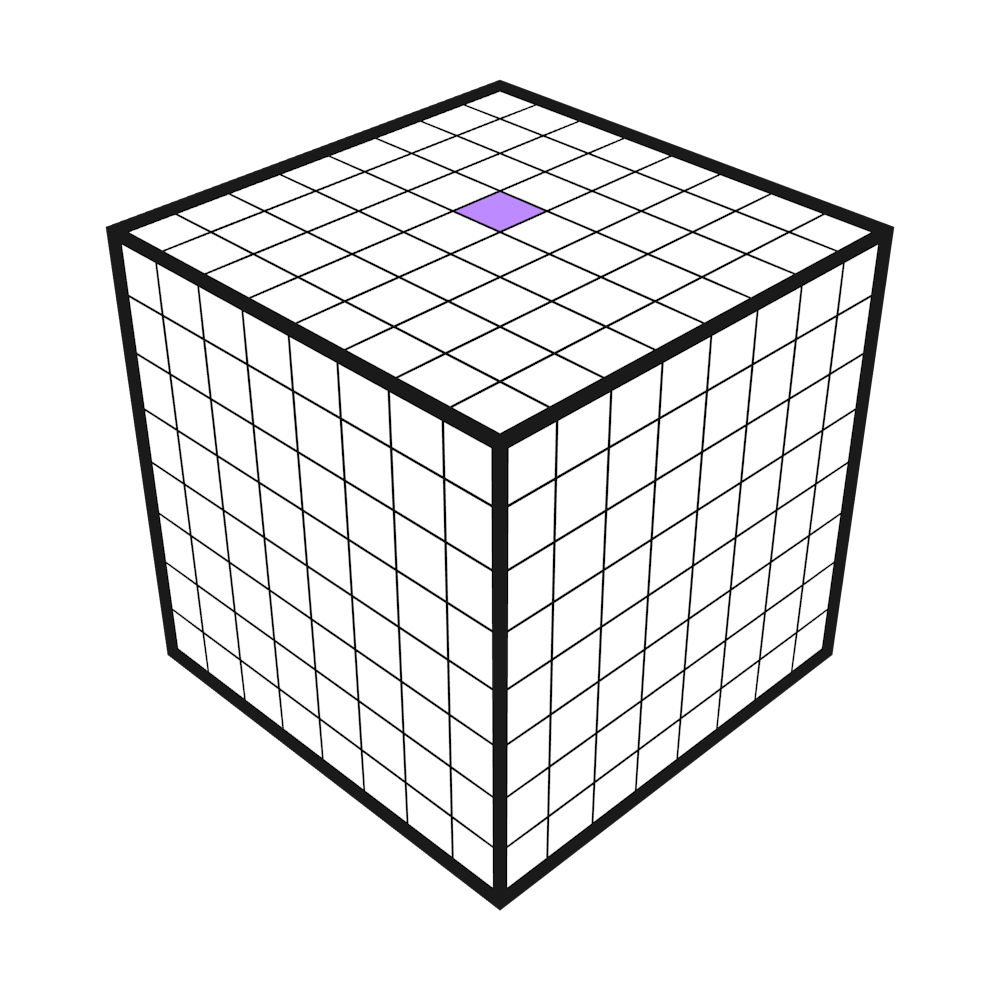
\includegraphics[width=3cm]{./img/raw/hs-datastructuren-overzicht/img3.png}};
\node[inner sep=0pt] (level_0) at (10.75cm,-2.75cm  - 1.5cm)
    {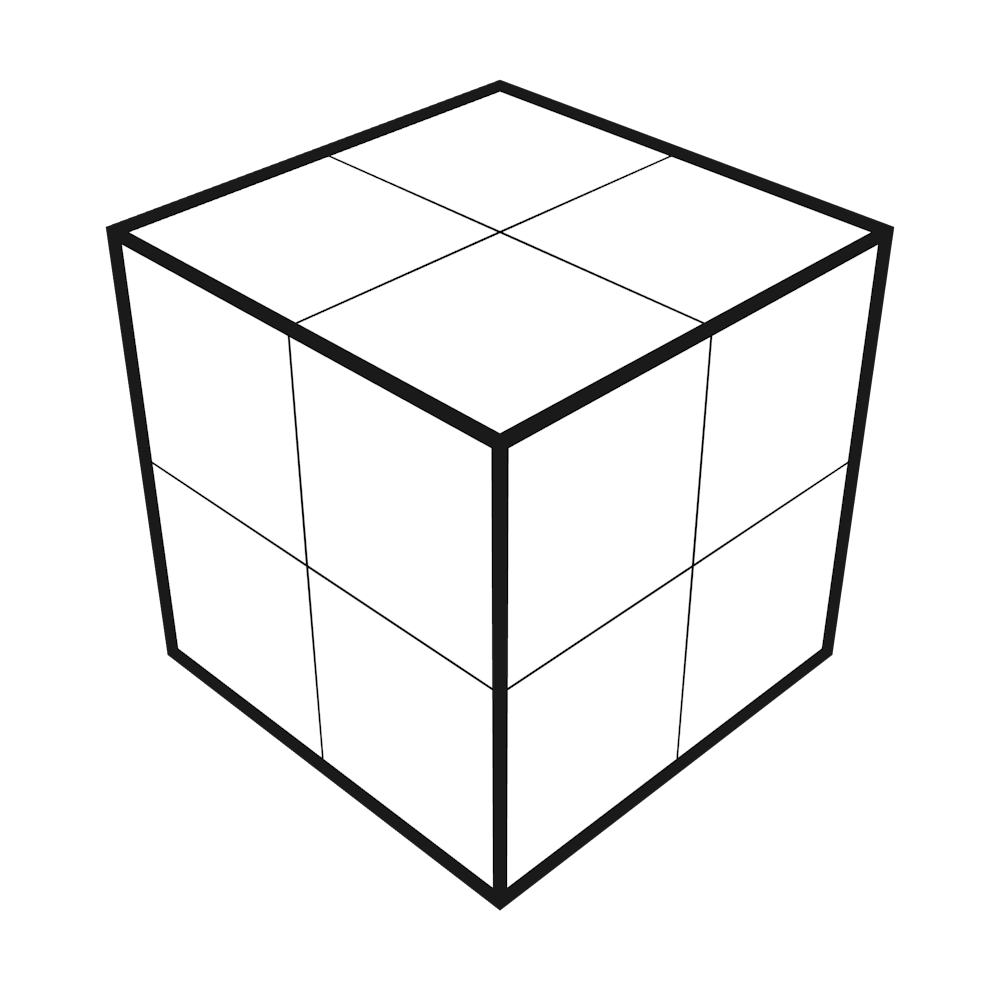
\includegraphics[width=2cm]{./img/raw/hs-datastructuren-overzicht/img2.png}};

\node[inner sep=0pt] (level_0) at (4.0cm,-3cm - 3.75cm  - 1.5cm)
    {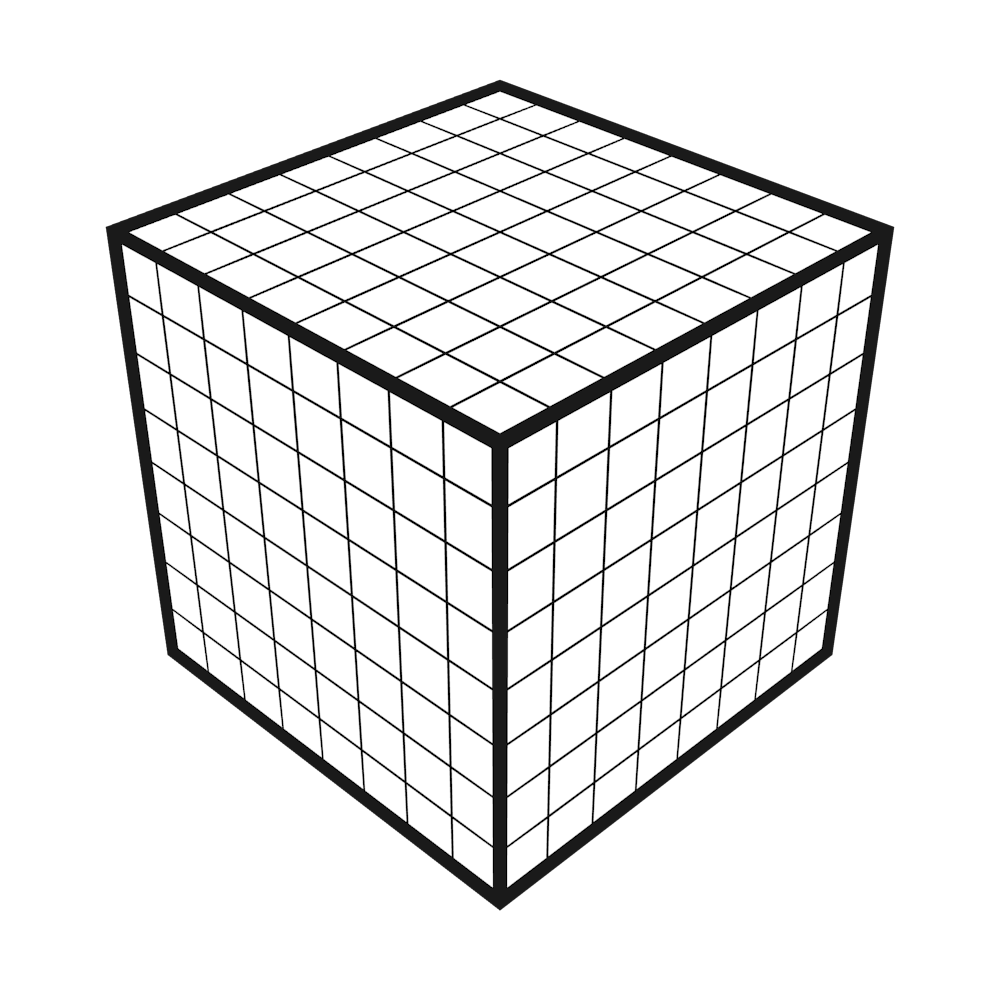
\includegraphics[width=3cm]{./img/raw/hs-datastructuren-overzicht/img1.png}};
\node[inner sep=0pt] (level_0) at (6.25cm,-2.75cm - 3.75cm  - 1.5cm)
    {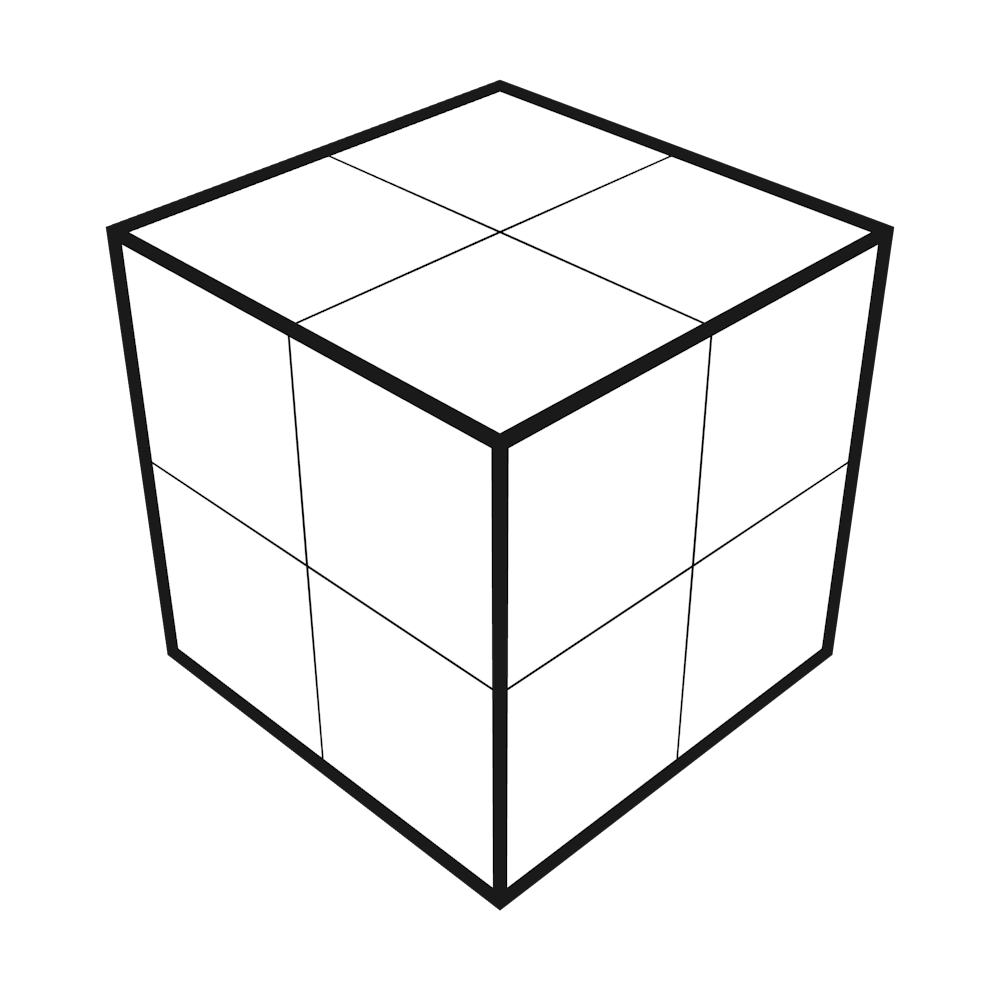
\includegraphics[width=2cm]{./img/raw/hs-datastructuren-overzicht/img2.png}};
\node[inner sep=0pt] (level_0) at (8.5cm,-3cm - 3.75cm  - 1.5cm)
    {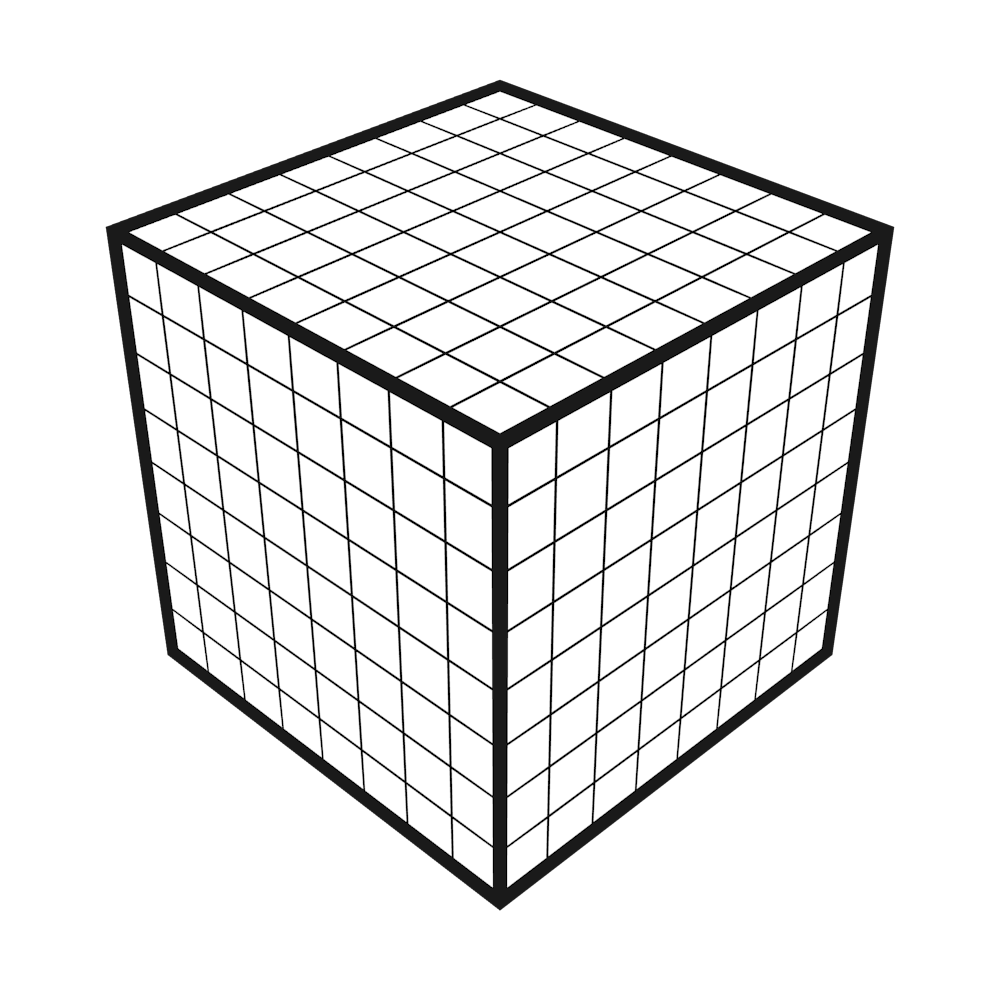
\includegraphics[width=3cm]{./img/raw/hs-datastructuren-overzicht/img1.png}};
\node[inner sep=0pt] (level_0) at (10.75cm,-2.75cm - 3.75cm  - 1.5cm)
    {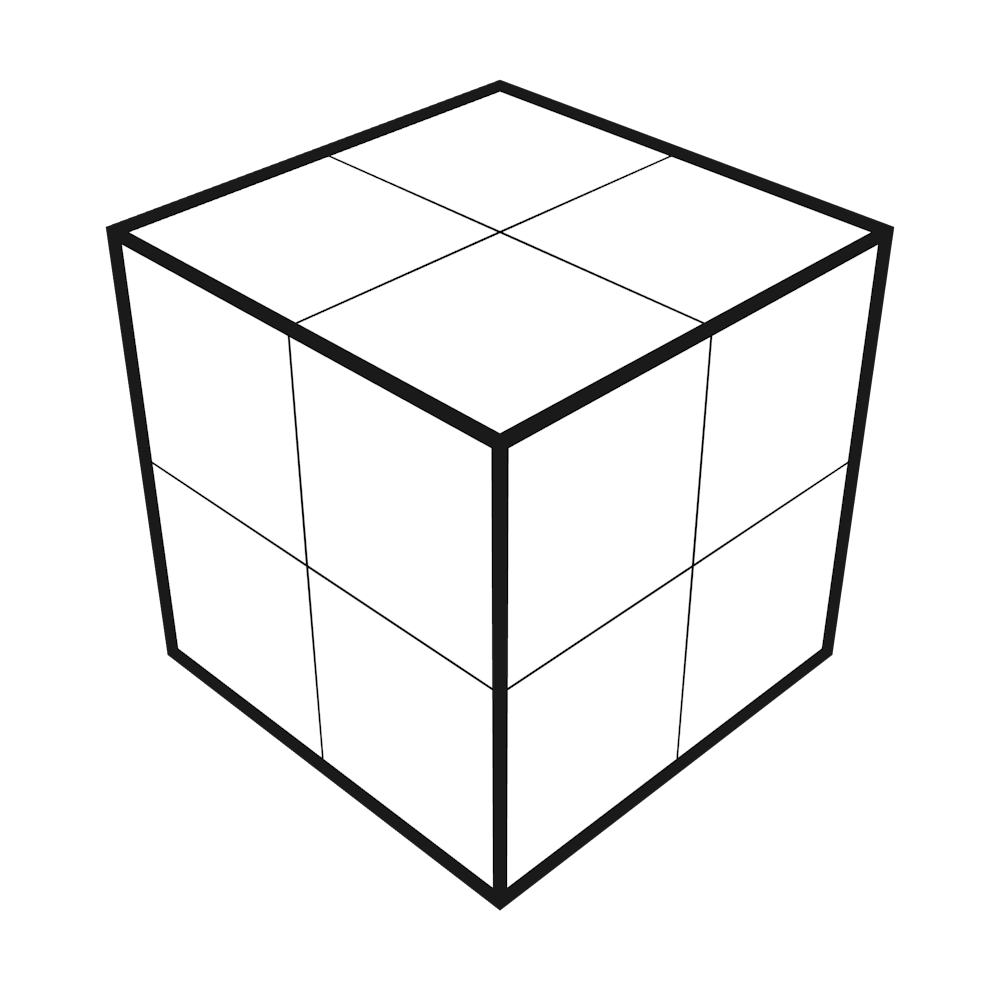
\includegraphics[width=2cm]{./img/raw/hs-datastructuren-overzicht/img2.png}};

\node at (11.75cm, -2.8cm) {\scriptsize layer $i$};
\node at (11.75cm, -2.8cm - 3.75cm) {\scriptsize layer $i + 1$};

\node at (3.0cm, -3.25cm) {$H_{1,i}$};
\node at (5.75cm, -3.25cm) {$\Phi_{1,i}$};
\node at (7.5cm, -3.25cm) {$H_{2,i}$};
\node at (10.25cm, -3.25cm) {$\Phi_{2,i}$};

\node at (3.0cm, -3.25cm -3.75cm) {$H_{1,i + 1}$};
\node at (5.75cm, -3.25cm  -3.75cm) {$\Phi_{1,i + 1}$};
\node at (7.5cm, -3.25cm -3.75cm) {$H_{2,i + 1}$};
\node at (10.25cm, -3.25cm -3.75cm) {$\Phi_{2,i + 1}$};

\node at (2cm, -2.5cm) (l1) {};
\node at (12.75cm, -2.5cm) (l2) {};
\draw[-, gray, very thin] (l1) -- (l2);

\node at (2cm, -2.5cm  -3.75cm) (l1) {};
\node at (12.75cm, -2.5cm  -3.75cm) (l2) {};
\draw[-, gray, very thin] (l1) -- (l2);

\node at (2cm, -2.5cm  -3.75cm -3.75cm) (l1) {};
\node at (12.75cm, -2.5cm  -3.75cm -3.75cm) (l2) {};
\draw[-, gray, very thin] (l1) -- (l2);

\node at (8.35cm, -3.63cm) (l1) {};
\node at (8.625cm, -3.63cm) (l2) {};

    \node at (-2.25cm + 10.75cm, -2cm + 1.5cm) (node_big) [grid_element_big, fill=tile0] {};
    \node at (-3.25cm + 10.75cm , -2cm + 1.5cm) (grid_l) [] {};
    \node at (-1.25cm + 10.75cm, -2cm + 1.5cm) (grid_r) [] {};
    \draw (grid_l.center) -- (grid_r.center);
    \node at (-2.25cm + 10.75cm, -1.5cm + 1.5cm) [] { \Large offset: $\mathit{k}$ };
    \node at (-2.25cm + 10.75cm, -2.5cm + 1.5cm) [] { \Large size: $\mathit{1}$ };

    \node at (-3.25cm + 10.75cm, -3cm + 1.55cm) (node_big_1) {};
    \node at (-1.25cm + 10.75cm, -3cm + 1.55cm) (node_big_2) {};


    \draw[gray] (node_big_1.center) -- (l1.center);
    \draw[gray] (node_big_2.center) -- (l2.center);
    
    \draw[-latex] (node_big.west) -- (light_index_0.south);


  \end{tikzpicture}
  \end{adjustbox}

  \caption{Overview of the data structures of Hashed Shading.}
  \label{fig:hs-data-structures}
\end{figure}


The goal of the Hashed Shading algorithm is to reduce the amount of work
required to build the data structures between frames, in order to improve the
overall performance compared to Tiled and Clustered Shading. It does so by
dividing the scene space camera-independently. Thus the data structures can be
reused between frames even if the camera position changes.
The scene space is represented with an octree data structure. This representation
is both precise and memory efficient.

The used data structures are based on the data structured used within Tiled and
Clustered Shading:

\begin{itemize}
  \item Linkless octree
  \item Light index list
  \item Global light list
\end{itemize}

\noindent The linkless octree replaces the tiles and clusters in Tiled and Clustered
Shading respectively. It contains two integers per filled node, one that defines the
offset within the light index list, and one that defines the size of the set of
indices within the light index list.

In order to construct these data structures the following steps have to be executed:

\begin{itemize}
  \item Define the scene space subdivision.
  \item Calculate the influence of each light on the subdivision.
  \item Combine the influences into one single scene octree.
  \item Construct the linkless octree and light index list based on the scene octree.
\end{itemize}

\noindent The first step requires the origin of the octree and the total size to be
calculated. Once these values are specified it is possible to define the influence
of each light in the scene. The combination of these influences leads to a scene
octree which has to be represented as a linkless octree in order to be used
effectively on the GPU. Finally for each sample the set of relevant lights is calculated
by descending into the octree. These steps will be explained in more detail in the
following chapters.

\subsection{Specification of the Octree}

To construct the octree a minimum bounding box which will fit all the lights at any
point in time during the simulation, needs to be defined. The minimum and maximum
points that define this bounding box can either be set by a developer or calculated
based on the light volumes. In order to ensure small rounding errors do not affect
the octree, an offset is added to these points.

Once the bounding box has been defined the size of the octree can be calculated. The
developer is responsible for setting the size of the nodes in the deepest layer of
the octree. Based on this node size $\mathit{l}$, the size of the octree can be calculated.
Assuming that $\mathit{d}_i$ is the maximum length of any of the sides of the
bounding box, the number of layers is equal to the smallest value of $k$ for
which holds

\begin{equation*}
  \mathit{l} \cdot 2^k \geq \mathit{d}_i
\end{equation*}

\noindent The size of the octree is equal to $\mathit{l} \cdot 2^k$.
With the origin and size defined it is possible to assign the lights to this subdivision of
space.

\subsection{Per Light Construction}

\begin{figure}[t]
  \centering
  \begin{subfigure}[b]{.3\linewidth}
    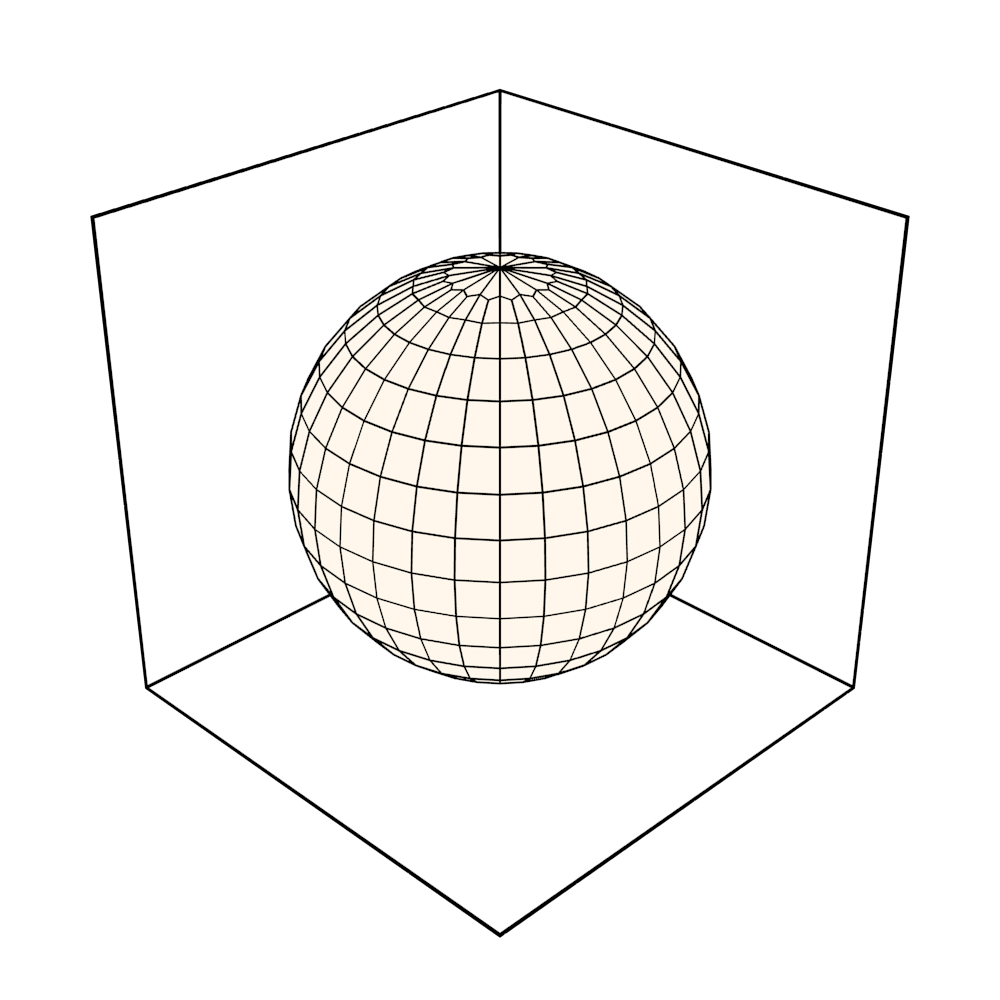
\includegraphics[width=\textwidth]{./img/raw/hs-slt-algorithm/hs-slt-algorithm-1.png}%
    \caption{\footnotesize Initial light volume}%
    \label{fig:hs-p1a}%
  \end{subfigure}
  %
  \begin{subfigure}[b]{.3\linewidth}
    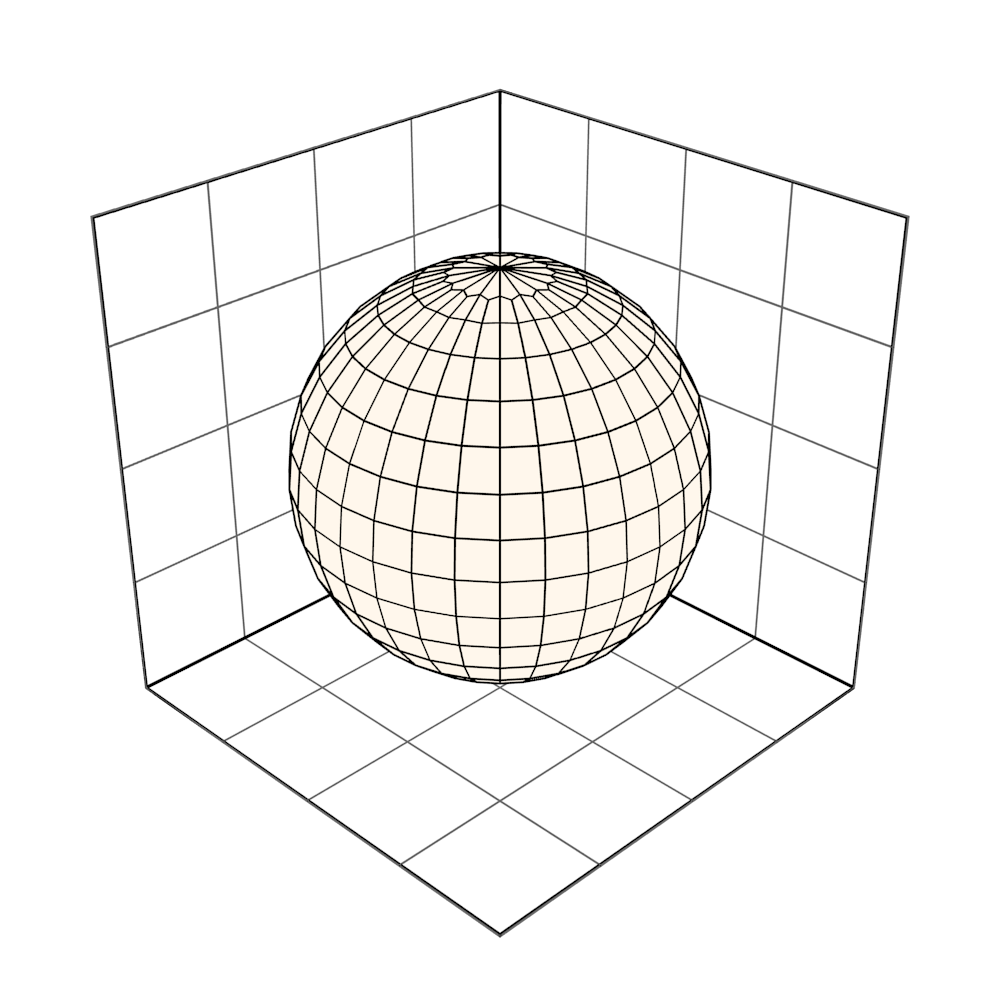
\includegraphics[width=\textwidth]{./img/raw/hs-slt-algorithm/hs-slt-algorithm-2.png}%
    \caption{\footnotesize Define grid}%
    \label{fig:hs-p1b}%
  \end{subfigure}
  %
  \begin{subfigure}[b]{.3\linewidth}
    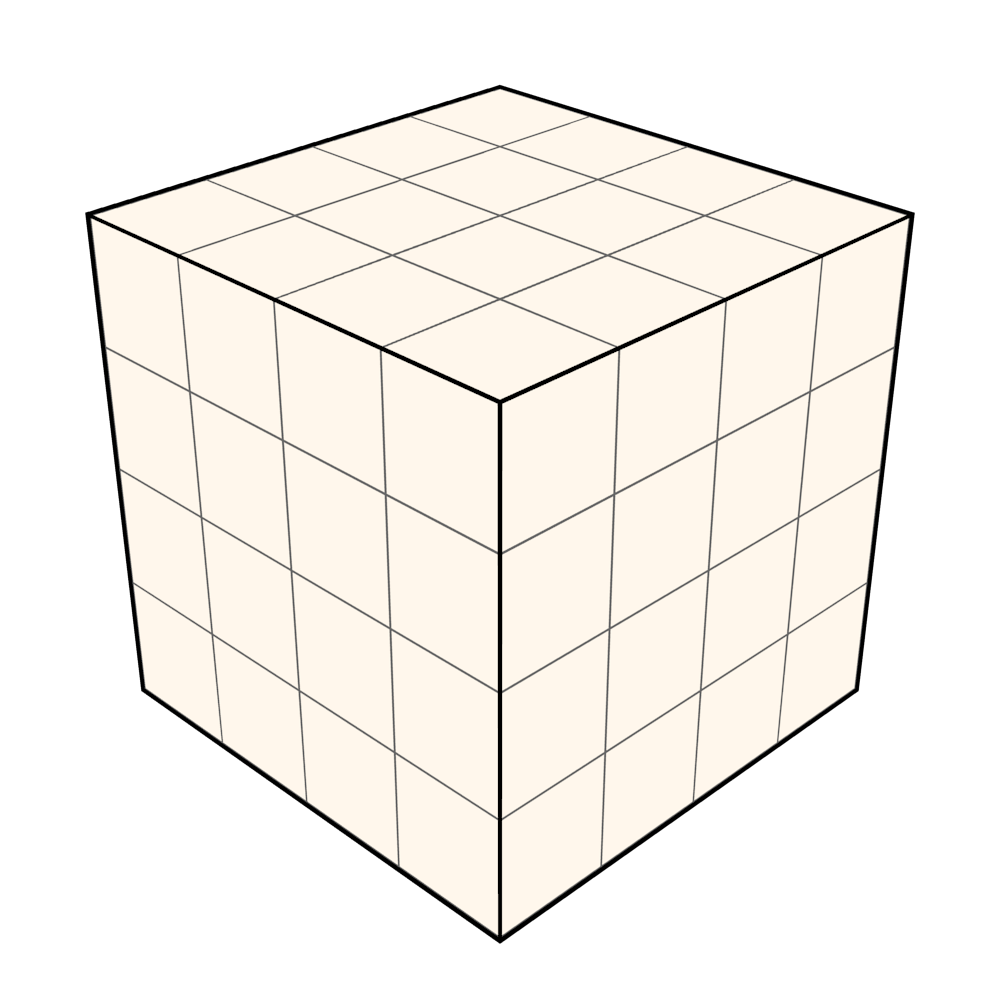
\includegraphics[width=\textwidth]{./img/raw/hs-slt-algorithm/hs-slt-algorithm-3.png}%
    \caption{\footnotesize Initialise grid}%
    \label{fig:hs-p1c}%
  \end{subfigure}
  \\
  \begin{subfigure}[b]{.3\linewidth}
    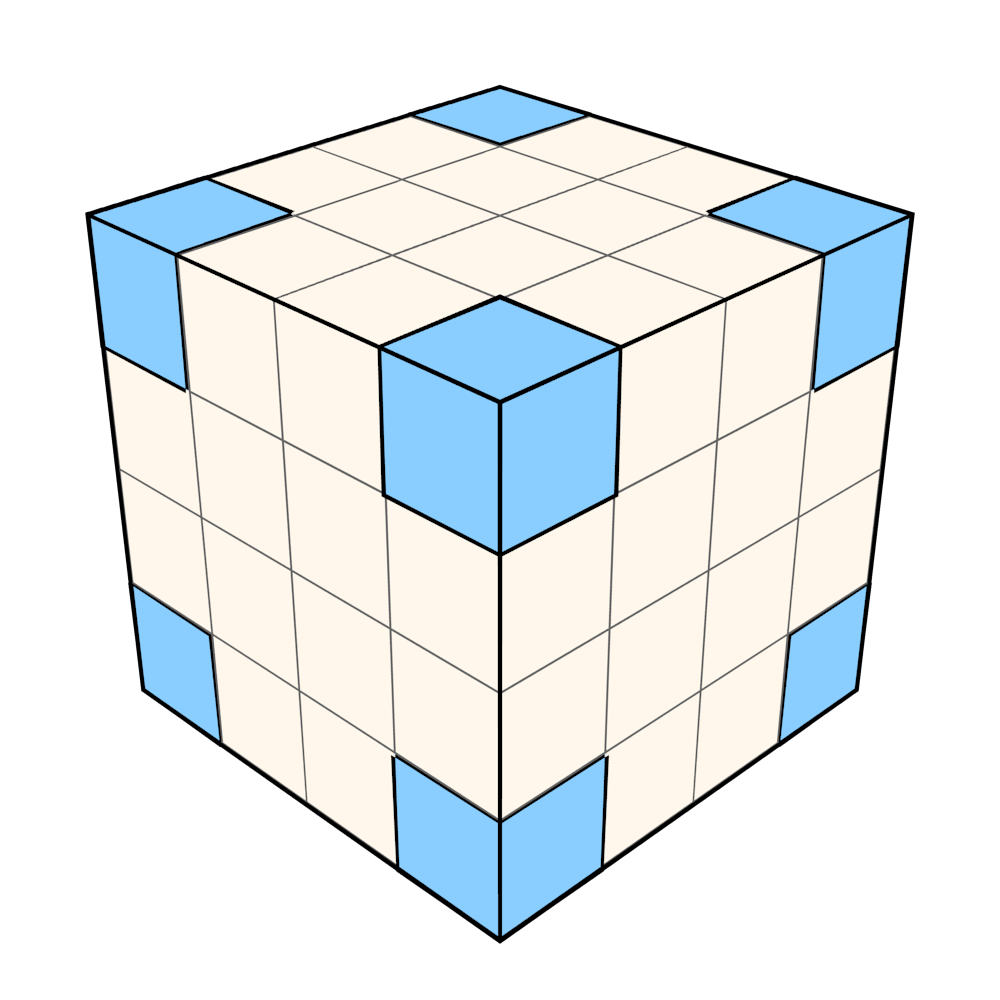
\includegraphics[width=\textwidth]{./img/raw/hs-slt-algorithm/hs-slt-algorithm-4.png}%
    \caption{\footnotesize Evaluate nodes}%
    \label{fig:hs-p1d}%
  \end{subfigure}
  %
  \begin{subfigure}[b]{.3\linewidth}
    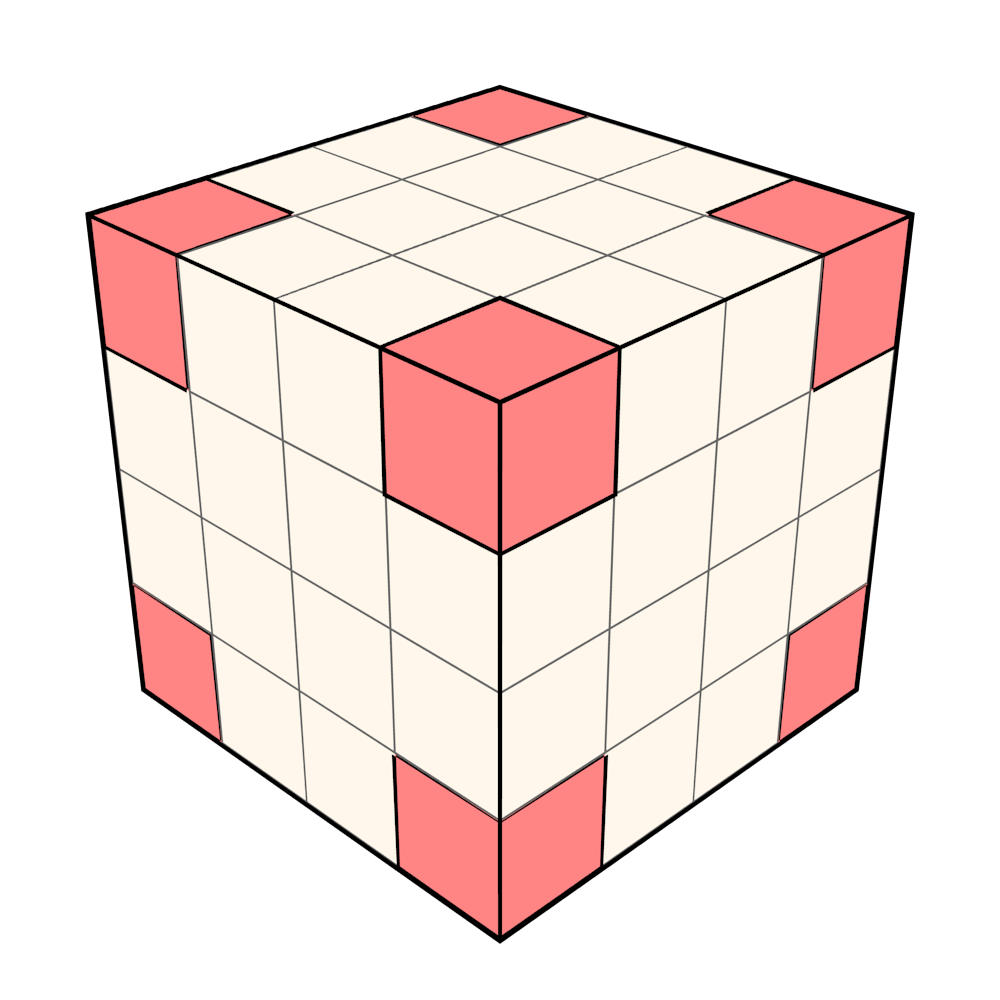
\includegraphics[width=\textwidth]{./img/raw/hs-slt-algorithm/hs-slt-algorithm-5.png}%
    \caption{\footnotesize Mark nodes}%
    \label{fig:hs-p1e}%
  \end{subfigure}
  %
  \begin{subfigure}[b]{.3\linewidth}
    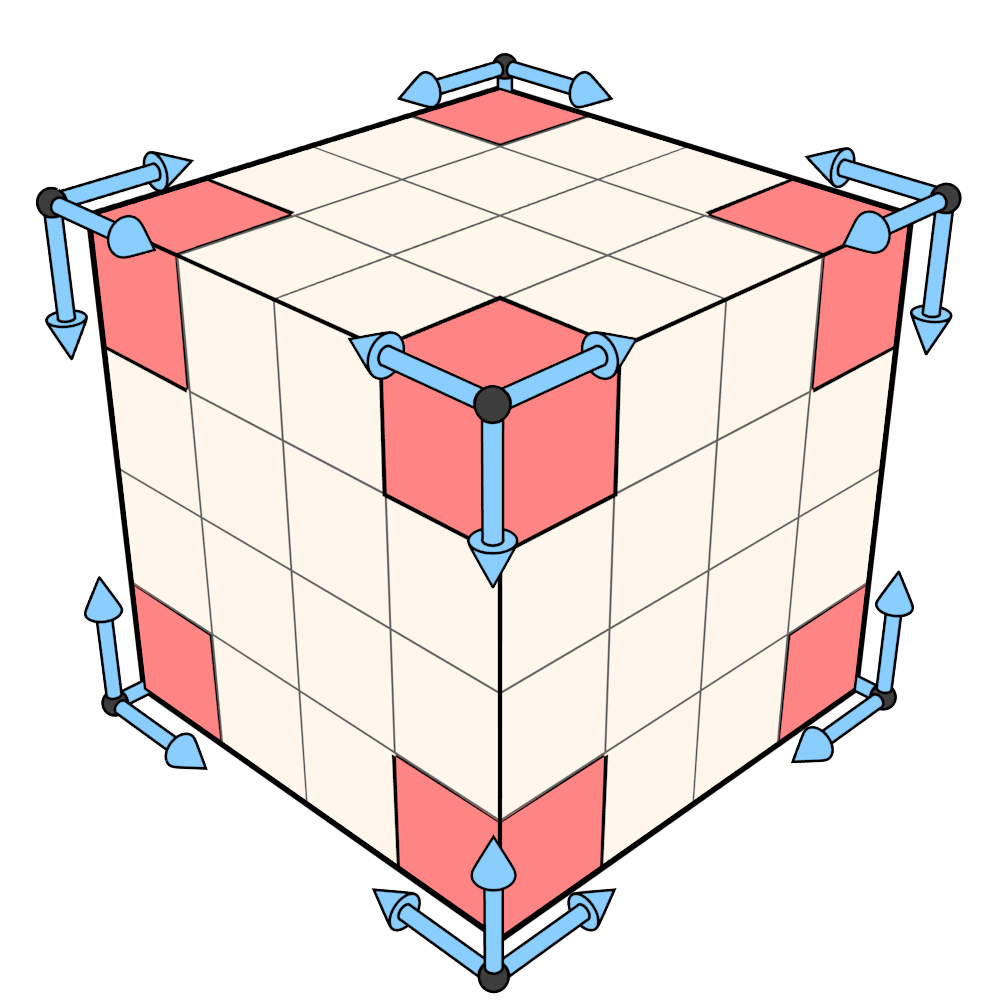
\includegraphics[width=\textwidth]{./img/raw/hs-slt-algorithm/hs-slt-algorithm-6.png}%
    \caption{\footnotesize Select nodes}%
    \label{fig:hs-p1f}%
  \end{subfigure}
  \\
  \begin{subfigure}[b]{.3\linewidth}
    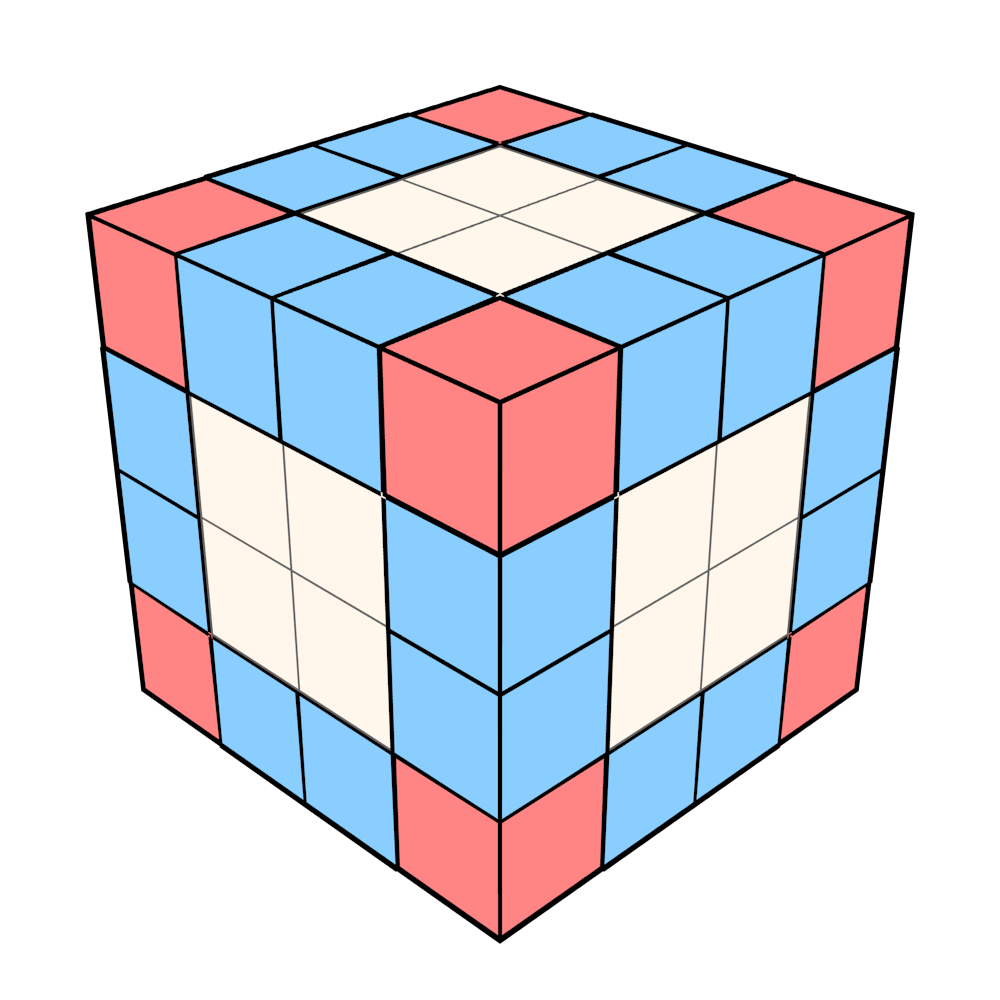
\includegraphics[width=\textwidth]{./img/raw/hs-slt-algorithm/hs-slt-algorithm-7.png}%
    \caption{\footnotesize Evaluate nodes}%
    \label{fig:hs-p1g}%
  \end{subfigure}
  %
  \begin{subfigure}[b]{.3\linewidth}
    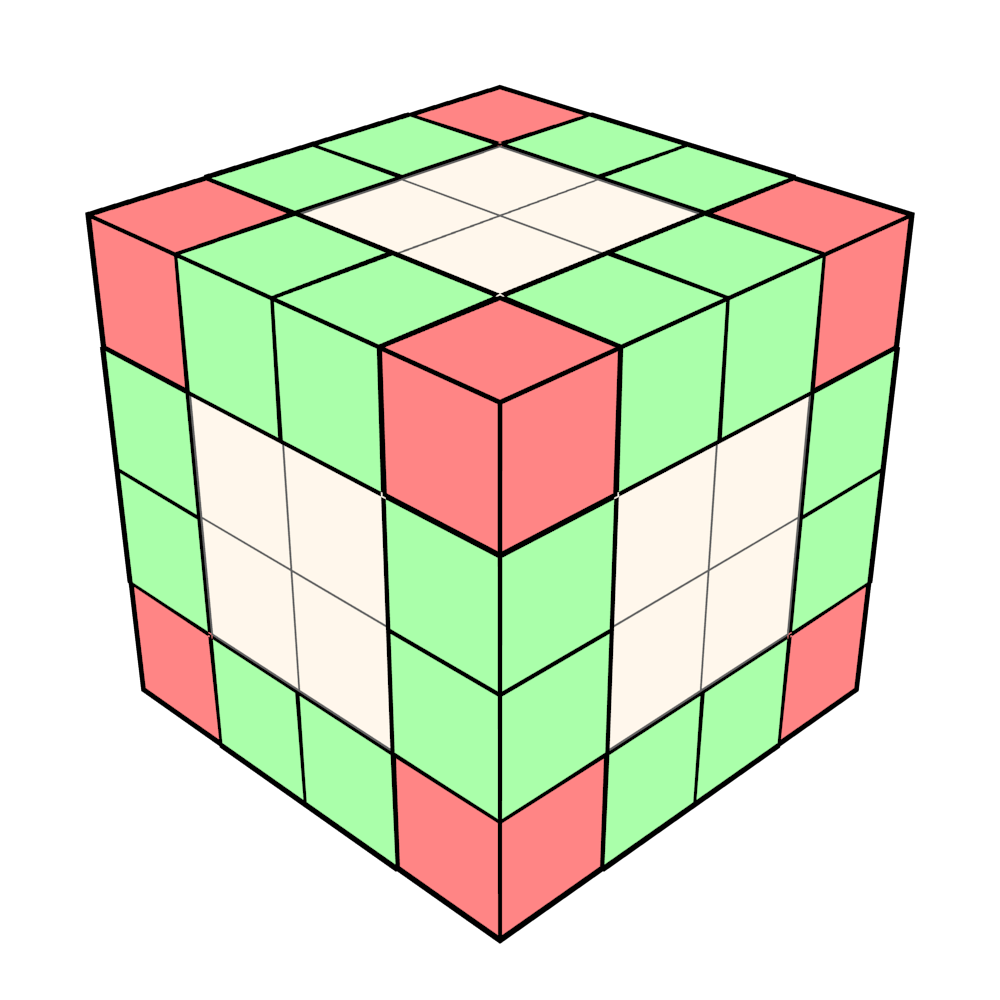
\includegraphics[width=\textwidth]{./img/raw/hs-slt-algorithm/hs-slt-algorithm-8.png}%
    \caption{\footnotesize Mark nodes}%
    \label{fig:hs-p1h}%
  \end{subfigure}
  %
  \begin{subfigure}[b]{.3\linewidth}
    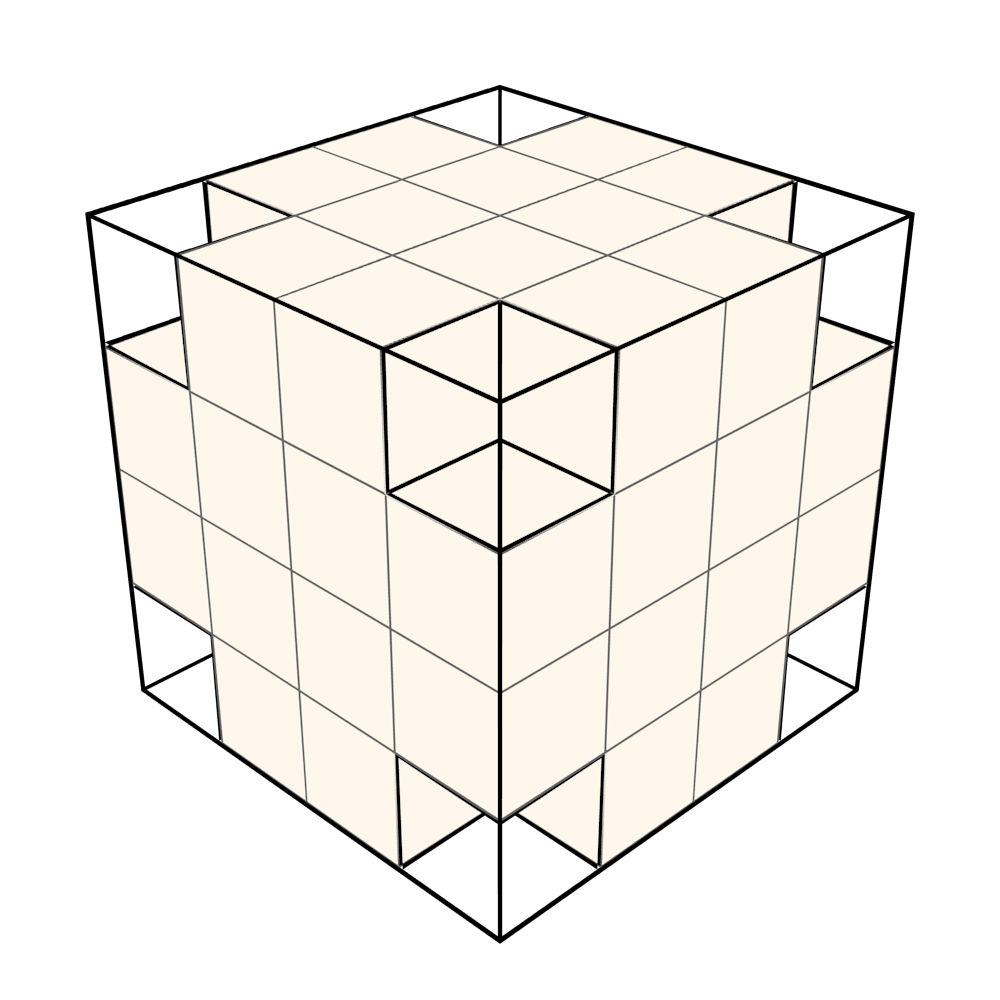
\includegraphics[width=\textwidth]{./img/raw/hs-slt-algorithm/hs-slt-algorithm-9.png}%
    \caption{\footnotesize Finalise grid}%
    \label{fig:hs-p1i}%
  \end{subfigure}

  \caption{Algorithm to determine the overlap of a single light with a grid of minimal nodes.}
  \label{fig:hs-p1}
\end{figure}


We only consider point lights within the current implementation of the algorithm. In order to
support different light types, a similar approach need to be developed for these lights, such
that the influence they have on the scene space subdivision can be efficiently calculated.

Any light has an influence on a node if the light volume overlaps with the node volume. In case
of point lights this can be easily calculated by comparing the distance between the light origin
$\mathbf{l}\mathtt{.orig}$ and the point inside the node volume closest to the light origin $\mathbf{p}$,
and the radius of the point light $\mathbf{l}\mathtt{.radius}$
volume. In case this distance is smaller than the radius, the node volume overlaps with the light
volume:

\begin{equation*}
  \left\lVert \mathbf{p} - \mathbf{l}\mathtt{.orig} \right\rVert < \mathbf{l}\mathtt{.radius}
\end{equation*}

\noindent Point $\mathbf{p}$ within the node volume and closest to the light origin can be easily
calculated by clamping the light volume per dimension between the extreme values of the node:

\begin{equation*}
  \mathbf{v} = \begin{pmatrix} \mathbf{l}.\mathtt{orig}_x \vert_{\mathbf{n}_{x}, \mathbf{n}_{x} + \mathit{l}} \\
                               \mathbf{l}.\mathtt{orig}_y \vert_{\mathbf{n}_{y}, \mathbf{n}_{y} + \mathit{l}} \\
                               \mathbf{l}.\mathtt{orig}_z \vert_{\mathbf{n}_{z}, \mathbf{n}_{z} + \mathit{l}} 
\end{pmatrix} 
\end{equation*}

\noindent where $\mathbf{n}$ is the origin of the node.

This calculation does not need to be executed for every node within the scene space.
Any node overlapping with the light lies within the minimal grid of nodes which contains the light volume.
Furthermore, each light is uniform, meaning that once we have established the boundaries of overlapping
and non-overlapping nodes, we know of all nodes whether they are overlapping or not.
This can be exploited by using a flood-fill algorithm to either fill the empty or overlapping nodes.

Because the volume of a sphere is slightly bigger than half its bounding box and because partly
overlapping nodes are also considered non-empty, we start with the assumption that each node
is overlapping, and fill the non-overlapping nodes. We use a breadth-first flood fill algorithm,
where each of the corner nodes of the grid are the seed nodes. If a node overlaps it is marked as
checked and removed from the queue. If a node does not overlap it is marked as checked and the
three nodes adjacent to the node facing inwards are added to the queue if they have not been checked
before. This is process is shown in figure \ref{}.
Once the queue is empty, all overlapping nodes have been determined.

\begin{figure}
  \centering
  \begin{subfigure}[b]{.45\linewidth}
    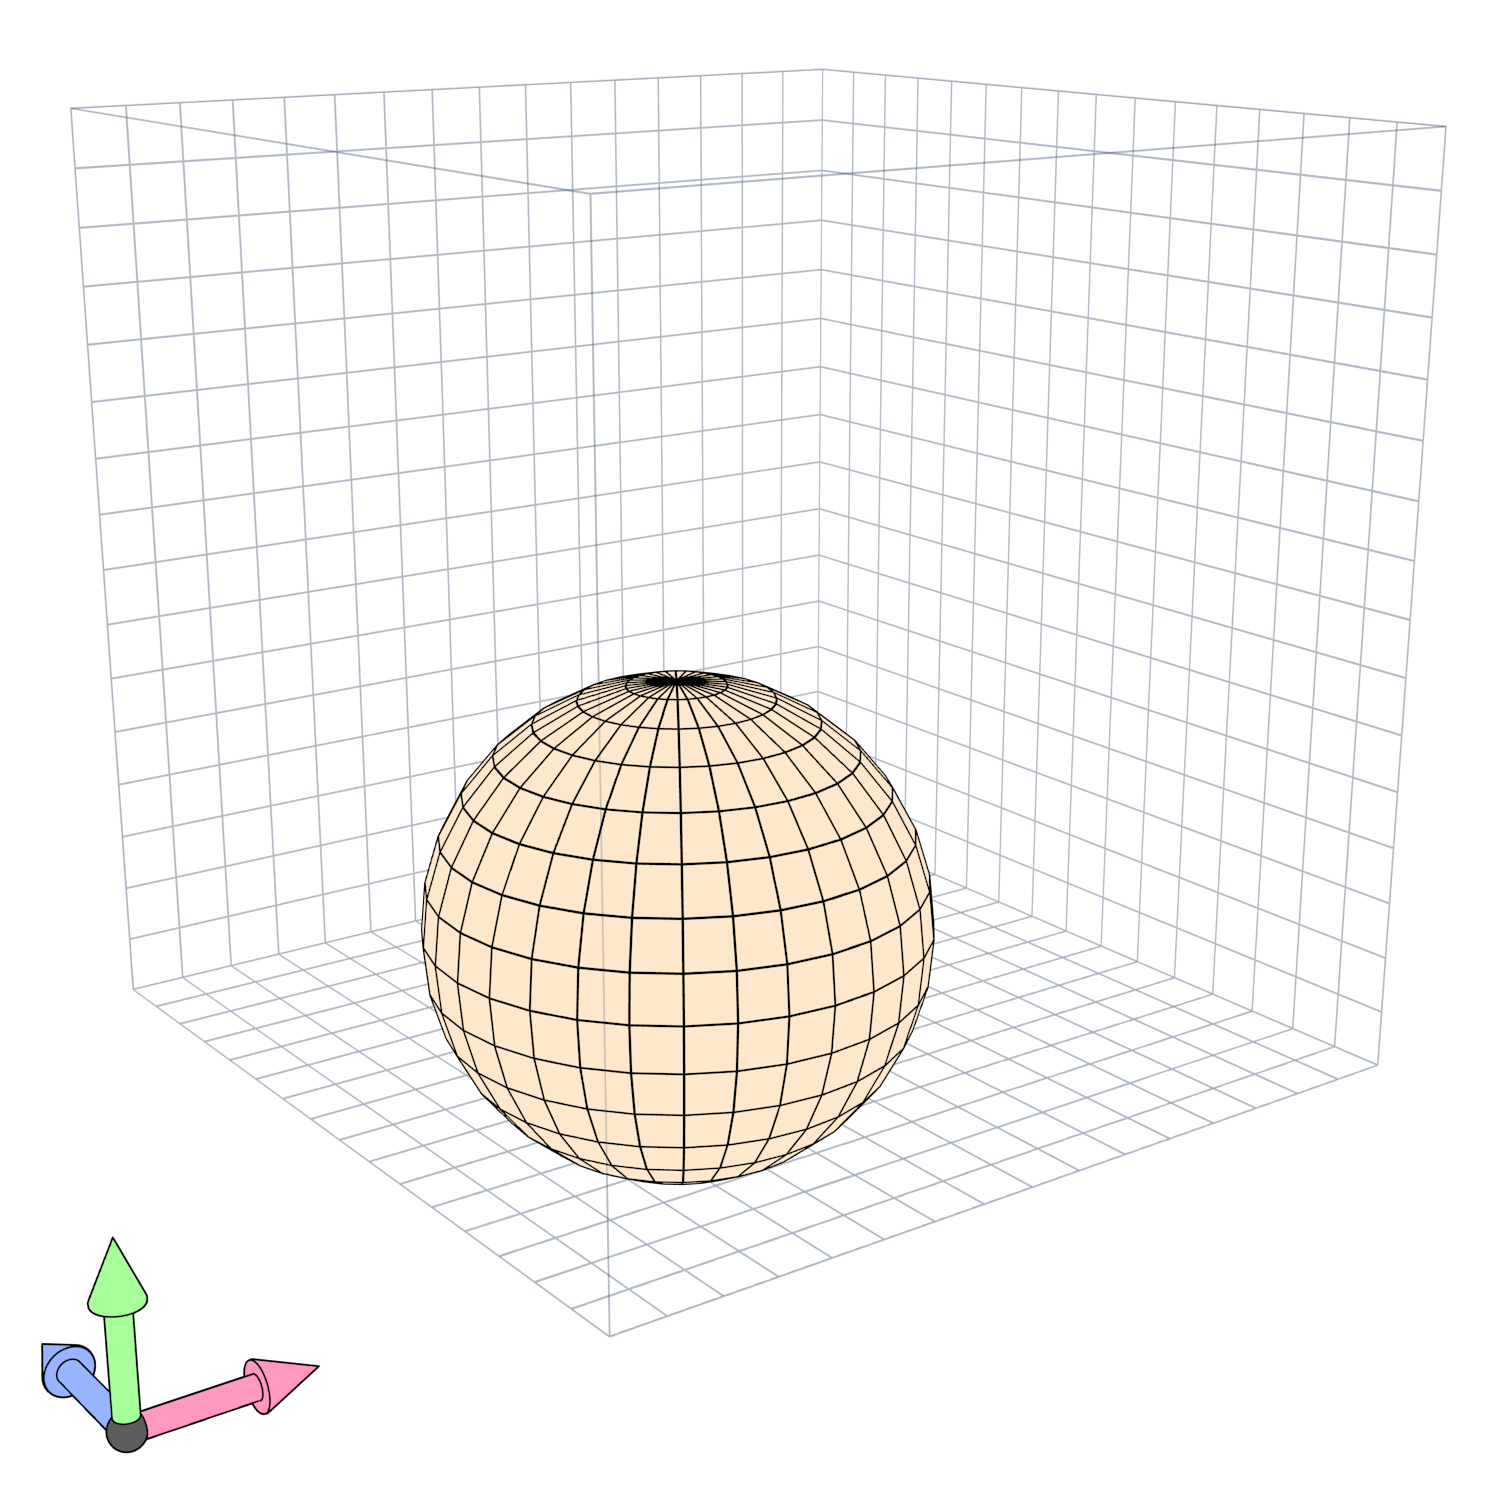
\includegraphics[width=\textwidth]{./img/raw/hs-slt/hs-slt_left.png}%
    \caption{Light volume}%
    \label{fig:hs-slt-left}%
  \end{subfigure} %
  \begin{subfigure}[b]{.45\linewidth}%
    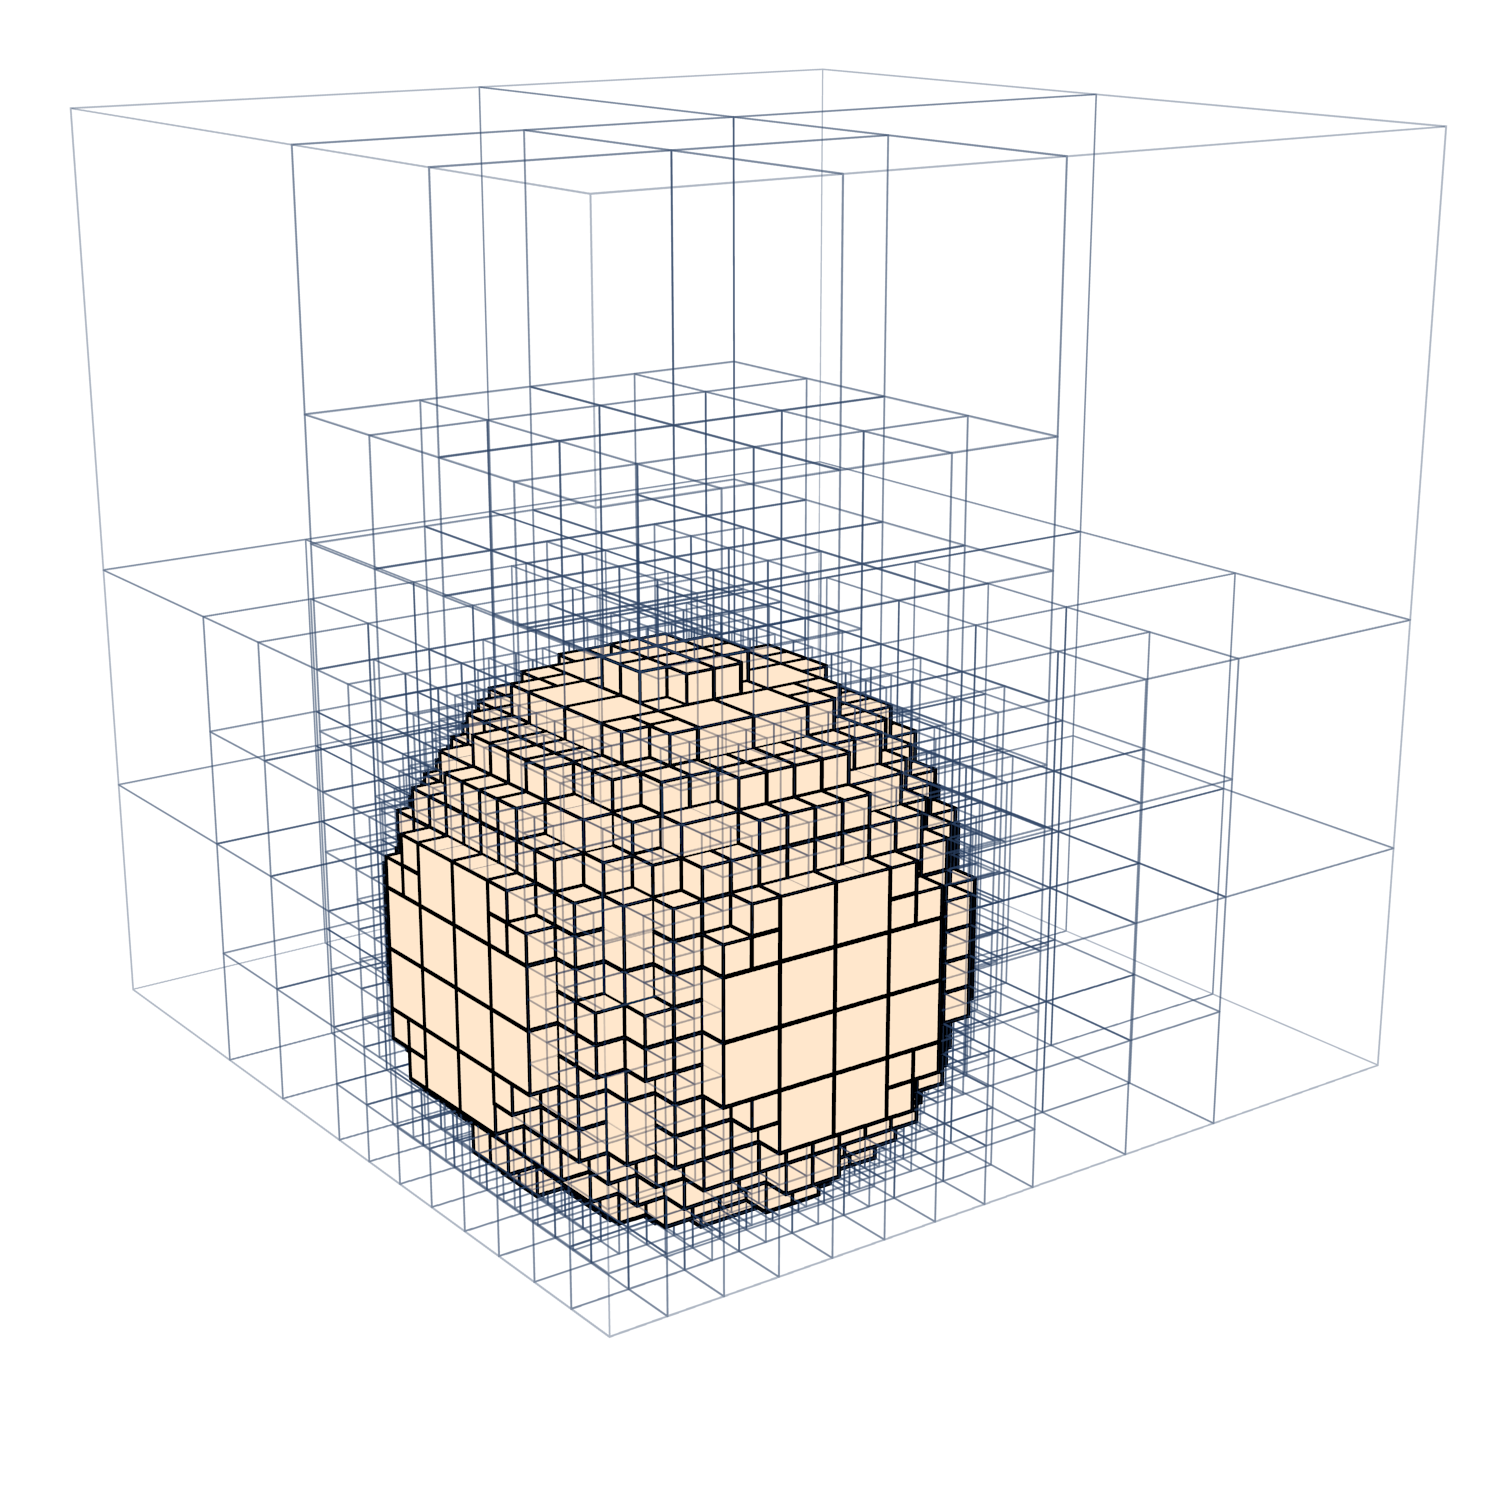
\includegraphics[width=\textwidth]{./img/raw/hs-slt/hs-slt_right.png}%
    \caption{Octree subdivision}%
    \label{fig:hs-slt-right}%
  \end{subfigure}
  \caption{Octree representation of a single light volume.}
  \label{fig:hs-slt}
\end{figure}


Finally the way these lights are represented in memory needs to be considered. If a light is
static during a whole simulation, there is no need to save the explicit influence of the
light separately and the overlapping nodes can all be combined in the scene octree.
However when a light is dynamic, the changing influence of the light on the subdivision of
the scene space needs to be calculated. This can be done efficiently by comparing the nodes
a light influences in the previous and current frame. Thus it is necessary to efficiently
represent each dynamic light in memory, in order to save computation time.
When the lights are small, or the node size is large, the grid could be saved directly in
memory. However when the node size is small compared to the point light radius, this leads
to unnecessary memory usage. The grid can be represented more compact by converting it into
an octree as well. This can be done in a top-down fashion by making use of the grid.
First the octree node which fully contains the grid is calculated. This node will serve
as a root node. For each node there are initially three possible options. The grid
does not overlap with the node, in which case the node is empty, as no overlapping nodes
lay outside of the grid. The grid partially overlaps with the node and the node falls
within the grid.

When the node overlaps partially there are two possibilities. Either the grid node
in the octree node closest to the light origin is overlapping, or it is not.
If it is, then the octree node is a branch node, and the eight children are evaluated.
If the grid node does not overlap with the light volume, the octree node is empty
as well.

In the last case there are three possibilities. If the grid node within the octree
node volume closest to the light origin is empty, the octree node will be empty
as well. If the closest grid node overlaps with the light volume, then either
the grid node within the octree node volume furthest from the light origin overlaps
with the light volume or it does not. In case it overlaps as well, then the whole
octree node volume overlaps, and thus the octree node is an overlapping leaf node.
If the furthest grid node does not overlap, the octree node contains both overlapping
and non-overlapping nodes, and the octree node is a branch node. The children of
this octree node are subsequently evaluated.

\subsection{Construction of the Scene Octree}

The scene octree is an octree structure of which the leaf nodes contain references
to the lights which overlap with the leaf node volumes. Depending on the representation
of the single lights, the scene octree can be constructed either top-down or bottom-up.

In case the lights are represented by the grid nodes which overlap with the light volume,
the nodes need to be combined first. This creates a set of nodes of minimum size that contain a set of
references to lights that overlap with these nodes. These can then be used to construct
the octree bottom-up. If the eight sibling nodes are leaf nodes and contain the same set of indices, it can
be replaced by a single leaf node in a higher layer, else a branch node in the layer above can be
added.

In case an octree representation is used, the scene octree can be build top-down by
recursively adding the light octrees to the scene octree. For each light octree the
scene octree node corresponding with the root of the light octree is found. Then the nodes
of the light octree are recursively added, where the filled light octree nodes are added
by adding the corresponding light index to the scene octree leaf node.

\subsection{Construction of the Linkless Octree and Light Index List}

As described in the overview, the octree nodes will specify a subset of the light index list.
Because this data is only saved in the leaf nodes of the scene octree. We opted for the
linkless octree variant that saves the data of the octree nodes separately from the octree
structure. Thus per layer a maximum of two spatial hash functions is constructed.

In the first step of construction of the linkless octree and light index list, the scene
octree nodes at the specified starting depth are gathered. For each of these nodes the
octree structure value is calculated as is specified in the algorithm of the linkless octree.
For each node we save whether the node is a leaf node, and whether the node contains any
information. If a node contains information, this information is stored in the second
spatial hash function. For each non-empty leaf node, the length of light index list
is saved, then the indices associated with the leaf node are added to the light index list.
The value saved in the second spatial hash function specifies the offset, equal to the length
of the light index list before adding the indices, and the length of the set of light indices.

\subsection{Light Assignment during Shading}

The final step of the algorithm is to use the constructed data structures to determine the set
of relevant lights per sample during the shading step. This step is similar to the shading
step of both Tiled and Clustered Shading. In order to find the subset of indices within the
light index list for a sample, we need to descend into the octree. For each layer we
calculate the octree structure of the node in which the sample falls. If this is a branch node,
the next layer is calculated. If the scene octree node is an empty leaf node, a vector containing
two zeroes is returned. If the the scene octree node is non-empty, the corresponding value is
obtained from the second spatial hash function of the current layer. The found offset and length
are returned.

Once the offset and length are obtained, the algorithm loops over the light indices within
the light index list, and for each light calculates the light contribution to the sample.
These values are summed and saved for the particular sample.

